\chapter{Evaluation}
\label{cha:evaluation}

%Having built the equivalent of a experimental setup, it is time to use
%the implementation to test the hypotheses.
%
%This is usually broken down in stages and subquestions.
%
%A structured approach to performing and reporting on experiments is
%to follow this pattern for every single experiment:
%
%\begin{enumerate}
%\item What is the purpose of the experiment?
%\item What is the expected outcome?
%\item What are the parameters under which the experiment takes place?
%\item What are the results?
%\item How do the results align with the expected outcome? If they do
%  not align, why is that so?
%\end{enumerate}
%
%Results should be presented summarised in tables and graphs.  Remember
%to note the number of times experiments were repeated, as well as
%averages, and standard deviations (in percent of the mean).  There is
%much more to the proper evaluation of experimental data than can be
%expounded upon here, but I turn the reader's attention to
%\citep{Downey2011:TSPASFP2011}, which is freely available.

In this chapter the implemented SeriChat prototype is evaluated with respect to the presented design goals. 

\section{Load Distribution}
One of the goals was to build a fair P2P system which make a fair load-balance between nodes in the network. It was expected that the root would have the most load among the group members. However, the results from the load distribution experiment shows, as illustrated in \autoref{fig:loaddistribution}, that the members in average has larger load than the root.

The experiment was done using 15 nodes running the SeriChat prototype. Five of the nodes (including the root) were members of the group and the rest were non-members. In the experiment the five members sent messages with an interval of one second for a total time of 10 minutes. The load is then calculated using a counter, which counts every request each has received.
\begin{figure}[!h]
	\centering
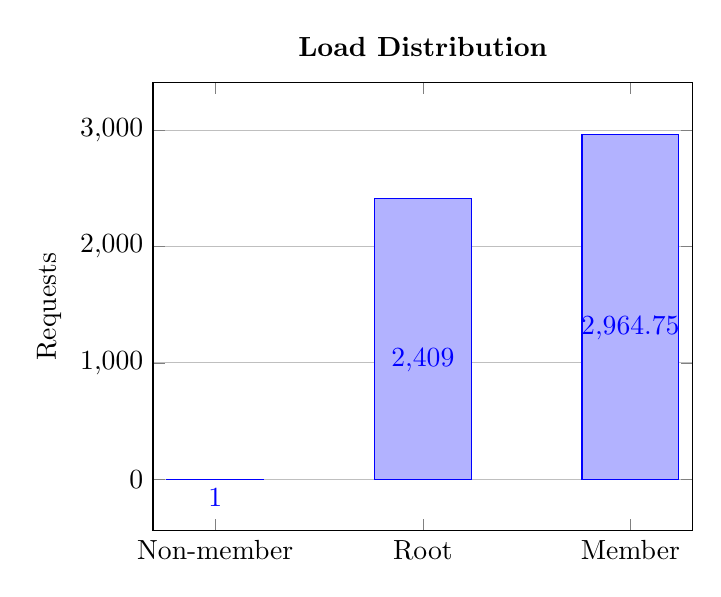
\begin{tikzpicture}
\begin{axis}[
title={\textbf{Load Distribution}},
ybar stacked,
%ymax=50,
ymajorgrids,
bar width=35pt,
%width=250pt,
nodes near coords, 
%nodes near coords={\pgfmathprintnumber\pgfplotspointmeta \%},
nodes near coords align={anchor=north},%Move values in bar
every node near coord/.style={
},
enlargelimits=0.15,
legend style={at={(0.5,-0.20)},
	anchor=north,legend columns=-1},
%width=0.8*\textwidth,
ylabel={Requests},
symbolic x coords={Non-member, Root, Member},
xtick=data,
%legend pos= north east,
%x tick label style={rotate=45,anchor=east},
]
%ethernet
\addplot+[ybar] plot coordinates {(Non-member,1) (Root,2409) 
	(Member,2964.75) };
%\legend{\strut Ethernet}
\end{axis}
\end{tikzpicture}
\caption{Results for load distribution} \label{fig:loaddistribution}
\end{figure}

We discovered that even though the root is loaded with the join requests, the root saves some load, not having to receive its own messages, when forwarding messages. Whereas all the rest of the members also have to receive their own messages during forward.

\section{Message Delivery Latency}
Another goal was to be able to replace existing solutions and therefore it is important that SeriChat is fast and responsive. 
This experiment is intended to measure the latency between the time a root receives a message and the time when this message is received by all the members. 

The experiment was repeated three times using respectively 15, 25, and 80 nodes running the SeriChat prototype. 

The results from the message delivery experiment are, as illustrated in \autoref{fig:messagelatency}. Having in mind that a typical group chat won't have more than 80 members at a maximum, so a latency of 511 ms for a group with 80 member is not that bad. It should be noticed though that this experiment is made locally on one machine, but if it was to be used in a real distributed system the latency will naturally have been higher than these results.   

% pænt
%normal 10-25 antal i grypper --> 80 er en stor gruppe,  erfraing
%511 ms ikke så lang tid
%experiment made locally
%more latency in real distributed systems offcourse
%
\begin{figure}[!h]
	\centering
	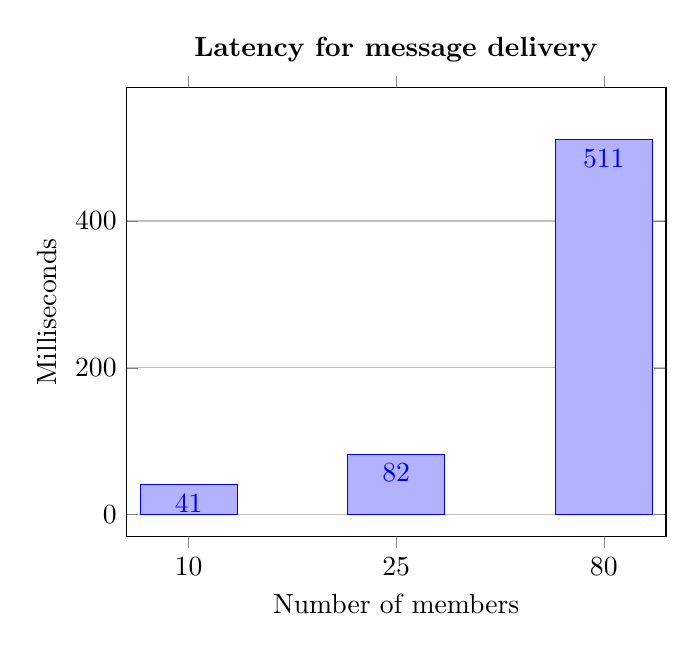
\begin{tikzpicture}
	\begin{axis}[
	title={\textbf{Latency for message delivery}},
	ybar,
	%ymax=50,
	ymajorgrids,
	bar width=35pt,
	%width=250pt,
	nodes near coords, 
	%nodes near coords={\pgfmathprintnumber\pgfplotspointmeta \%},
	nodes near coords align={anchor=north},%Move values in bar
	every node near coord/.style={ 
	},
	enlargelimits=0.15,
	legend style={at={(0.5,-0.20)},
		anchor=north,legend columns=-1},
	%width=0.8*\textwidth,
	ylabel={Milliseconds},
	xlabel={Number of members},
	symbolic x coords={10, 25, 80},
	xtick=data,
	%legend pos= north east,
	%x tick label style={rotate=45,anchor=east},
	]
	%ethernet
	\addplot+[ybar] plot coordinates {(10,41) (25,82) 
		(80,511) };
	
	%\legend{\strut Ethernet}
	\end{axis}
	\end{tikzpicture}
\caption{Results for message delivery latency} \label{fig:messagelatency}
\end{figure}